\documentclass{article}

% set font encoding for PDFLaTeX or XeLaTeX
\usepackage{ifxetex}
\ifxetex
  \usepackage{fontspec}
\else
  \usepackage[T1]{fontenc}
  \usepackage[utf8]{inputenc} % Permite escribir en español
  \usepackage{lmodern}
\fi

\usepackage{graphicx}

% used in maketitle
\title{Reporte de Actividad 1}
\author{Manuel Ignacio Gómez García}
\date{30 de enero, 2018}

% Enable SageTeX to run SageMath code right inside this LaTeX file.
% documentation: http://mirrors.ctan.org/macros/latex/contrib/sagetex/sagetexpackage.pdf
% \usepackage{sagetex}

\begin{document}

\maketitle ATMÓSFERA DE LA TIERRA

\section{Introducción}

La atmósfera de la Tierra está compuesta principalmente de gases, gracias a la gravedad del planeta. Es debido a la ella que existe la vida pues genera presión que da lugar al agua, nos protege de la radiación emitada por el Sol, disminuyendo así la cantidad y calentando la Tierra lo necesario.
\\
\\ El volumen de la atmósfera es un 78.09\% nitrogeno, 20.95\% oxígeno, 0.93\% argón, 0.04\% dióxido de carbono, y el resto corresponde a otro tipo de gases.
\\
\\ La atmósfera cuenta con una masa aproximadamente de $5.15x10^{18}$ kg, de los cuales $\frac{3}{4}$ se encuentran entre los primeros 11 km de la superficie. A lo largo de ella, conforme aumenta la altitud, podemos distinguir distintas capas y que son clasificadas en base a características como su temperatura y composición.

\section{Composición}

Los tres mayores constituyentes de la atmósfera son nitrógeno, oxígeno y argón, mientras quue el vapor de agua apenas representa el 0.25\%; su concentración varía alrededor de 10 ppm por volumen en las zonas más heladas hasta 5\% por volumen en las más calientes. Los gases restantes son rastros del efecto invernadero, siendo estos dióxido de carbono, metano, óxido nitroso, y ozono, así como otro tanto más de restos químicos provenientes de la contaminación de gases de origen natural, aerosoles, o bien, por las fábricas.

\section{Estructura de la atmósfera}

En general, la presión y densidad disminuye conforme aumenta la altitud,       sin embargo con la temperatura es algo más complicado que eso debido a que     se mantiene relativamente constante, por lo cual es necesario medir estos       cambios con ciertos dispositivos, en base a ello se ha dividido la             atmósfera en cinco distintas capas.

\begin{figure}
    \centering
    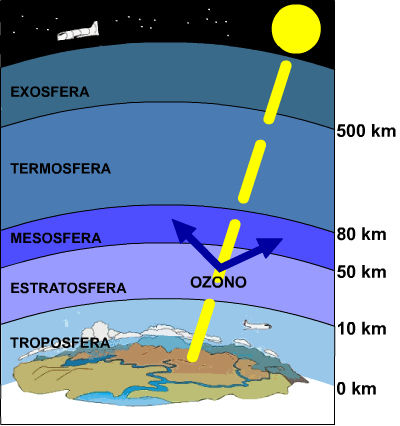
\includegraphics[width=5cm]{CapasAtmosfera}
    \caption{Capas de la atmósfera}
\label{Atmosfera}
\end{figure}

    \subsection{Troposfera}
    
    La troposfera es la capa de la atmósfera donde habitamos los seres             vivos y abarca cerca de los primeros 12 km de altitud, aunque está             altitud varía según la ubicación (9 km en los polos y 17 km en el               ecuador).
    \\
    \\ Aunque ocurren ciertas variaciones, la temperatura desciende                 conforme se asciende a través de la atmósfera ya que existe una                 transferencia de energía con la superficie del planeta. Contenida en           esta capa encontramos el 80\% de la masa atmosférica y dentro de los           primeros 5.6 km, el 50\% de la masa total, conviertiendo a ésta en la           capa más densa de todas.
    \\
    \\ Aquí es donde vuelan las aeronaves propulsadas por hélices.
    
    \subsection{Estratosfera}
    
    Esta capa comienza en la tropopausa y termina alrededor de los 50 o 55         km de altitud.
    \\
    \\ La presión atmosférica en el borde superior de la capa es $\frac{1}         {1000}$ de la presión a nivel del mar. Aquí es donde encotraremos la           capa de ozono, es donde se encuentra una alta concentración de este             gas, es por ello que en esta capa incremente la temperatura conforme la         altitud pues los rayos UV son retenidos por el gas provocando que la           temperatura asciende desde -60 ºC hasta 0 ºC en la parte superior.
    \\
    \\ Esta es el punto más alto a donde pueden llegar las aeronaves               impulsadas por jet.
    
    \subsection{Mesosfera}
    
    Siendo la tercer capa más alta y abarcando entre los 50 km (mesopausa)         hasta 80-85 km de altitud tenemos a la mesosfera.
    \\
    \\ Conforme se aumenta la altitud, la temperatura comienza a descender en       este punto, al punto de ser este el espacio más helado del planeta con una     temperatura promedio de -85 ºC.
    \\
    \\ En esta capa es donde se forman las nubes más altas, y también es donde     más se consumen los meteoritos al entrar en nuestra atmósfera. Este lugar       se encuentra tan alto que es inaccesible para aeronaves del tipo jet y         demasiado bajo para poner equipo orbital cerca. Esta zona es mayormente         donde navegan los equipos impulsados por cohetes.
    
    \subsection{Termosfera}
    
    Se extiende desde la mesopausa (alrededor de 80 km de altitud) hasta los       500-1000 km, esta variación es debido a la actividad solar.
    \\
    \\ En la termosfera aumenta a medida que nos alejamos de la Tierra y puede     llegar a los 1500 ºC, sin embargo dado a la baja densidad presente en esta     capa, la sensación no es verdaderamente significante, de hecho, las             moléculas viajan en promedio 1 km antes de colisionar con otra; por ello,       aunque las moleculas sean altamente energéticas no se sentirían caliente       al  contacto humano.
    \\
    \\ A esta altura órbita la estación espacial internacional, entre 350 y 420     km.
    
    \subsection{Exosfera}
    
    La exosfera es la última capa de nuestra atmósfera y abarca desde los 700       km hasta 10,000 km, donde se une al viento solar.
    \\
    \\ La capa está compuesta de extremadamente bajas densidades de hidrógeno,     helio y otras tantas más moléculas pesadas incluyendo nitrógeno, oxígeno y     dióxido de carbono. Las partículas pueden viajar cientos de kilometros sin     colisionar con otras, por ello la exosfera no se comporta como un gas,         además de que muchas partículas terminan saliendo al espacio exterior           debido a esto.
    \\
    \\ La mayoría de los satélites que orbitan la Tierra se ubican aquí.

\section{Propiedades físicas}

    \subsection{Presión y espesor}
    
    La presión atmosférica a nivel del mar es de 101325 Pascales, o bien, una atmósfera (1 atm). La masa atmosférica total es de $5.1480x10^{18}$ kg y una superficie de 51007.2 megahectareas. Debido a la naturaleza del paneta la presión  varía según la locación y climade dicha zona.
    \\
    \\ La densidad en la atmósfera no es uniforme, por lo cual conforme aumenta la altitud la presión disminuye exponencialmente, provocanco así una reducción a la mitad cada 5.6 km. Sin embargo, usualmente la presión atmosférica es modelada distinta según la capa que se tome a consideración, cada una toma en cuenta gradientes de la temperatura, composición molecular, radiación solar y gravedad.
    
    \subsection{Temperatura y velocidad del sonido}
    
    La división de la atmósfera es debido a la temperatura que experimenta. Desde el nivel del mar hasta los 11 km de altitud la temperatura deciende gradualmente, tras los 11 km se mantiene prácticamente constante durante una gran distancia vertical en el resto de la troposfera. Posteriormente, cerca de los 20 km, vuelve a incrementar debido a la captura de rayos UV por la capa de ozono.
    \\
    \\ En un gas ideal, la velocidad del sonido depende únicamente de la temperatura y no de la presión o densidad, siendo así como lo hace el sonido en nuestra atmósfera.
    
    \subsection{Densidad y masa}
    
    La densidad del aire a nivel del mar es alrededor $1.2 kg/m^{3}$. En realidad la densidad no es medida sino calculada en base de la temperatura, presión y humedad aplicando la ecuación de estado del aire. Esta densidad disminuye mientras la altitud incrementa. Dichas variaciones se modelan usando fórmulas barométricas.
    \\
    \\ En promedio, la totalidad de masa presente en toda la atmósfera es de $5x10^{15}$ toneladas. Según el Centro Nacional Americano para la Investigación Atmosférica, la cantidad tiene cierto rango debido al agua de $1.5x10^{15}$ kg, dependiendo de la presión en el área.
    
    
\section{Propiedades ópticas}

La radiación solar es la energía que recibe la Tierra del Sol. El planeta emite cierta radiación de vuelta pero nos es imperceptible. Parte de esta radiación es absorbida y otra reflejada por la atmósfera.
    
    \subsection{Dispersión}
    
    Cuando la luz pasa a través de la atmósfera, los fotones se dispersan en ella. Si la luz no interacciona con la atmósfera entonces podemos llamarle una radiación directa; en cambio, cuando los rayos de luz han sido dispersados por la atmósfera se le llama radiación indirecta. Es por ello que el cielo luce azul pues se debe a las ondas generados por esta interacción y la tonalidad roja es aquella que presenta menos dispersión.
    
    \subsection{Absorción}
    
    Las distintas moléculas absorben distintas longitudes de onda de radiación (i.e. $O_2$ y $O_3$, longitudes menores a 300 nm y $H_2 O$, mayores a 700 nm) . En el momento que un fotón es absorbido, la molécula responsable incrementa su energía, calentando así la atmósfera aunque también se enfría al emitir radiación.
    \\
    \\ El espectro que logra traspasar se encuentra entre los 400-700 nm y continua alrededor de los 1100 nm.
    
    \subsection{Emisión}
    
    La emisión es lo opuesto a la absorción, representa la emisión de radiación. Esta tendencia de emisión depende de la emisión de "cuerpo negro", es por ello que los cuerpos más calientes emiten más radiación, con longitudes de onda muy cortas; mientras que los más helados, emiten menos y en con una longitud muy grande.
    
    \subsection{Índice de refracción}
    
    El aire presenta un índice de refracción muy cercano pero superior a 1. Esto puede ocasionar que se doblen los rayos de luz y hacer ver objetos en el horizonte antes de que estén en la verdadera posición.
    \\
    \\ La temperatura es un factor que altera el índice de refracción, haciendo que sean más notorios sus efectos cuando el gradiente de temperatura es grande.

\section{Circulación}

Circulación atmosférica es el movimiento a gran escala del aire a través de la troposfera, y los medios por los cuales el calor se distribuye alrededor de la Tierra. Este gran movimiento varía año con año pero la estructura básica se mantiene prácticamente constante ya que está determinado por la rotación del planeta y la diferencia de radiación entre el ecuador y los polos.

\section{Bibliografía}
\indent --- Atmosphere of Earth. Consultado el 29 de enero, 2018.
\\ \indent https://en.wikipedia.org/wiki/Atmosphere $_$ of $_$ Earth
\\
\\ --- Figura 1.
\\ \indent https://programacion167.files.wordpress.com/2016/08/2-atmosfera.png?w=700

\end{document}
